\documentclass[a4paper,10pt]{article}

\usepackage[margin=1in]{geometry} 	% Setea el margen manualmente, todos iguales.
\usepackage[spanish]{babel} 		% {Con estos dos anda
\usepackage[utf8]{inputenc} 		% todo lo que es tildes y ñ}
\usepackage{fancyhdr} 			%{Estos dos son para
\usepackage{ulem}
\pagestyle{fancyplain} 			% el header copado}
\usepackage{color}			% Con esto puedo hacer la matufia de poner en color blanco un texto para engañar al formato
\usepackage{graphicx}	% Para insertar gráficos
\usepackage{array}			% Para usar arrays
\usepackage{hyperref}		% Para que tenga links el índice

%\usepackage{datetime}	% Para agregar automáticamente fecha/hora de compilación y otras cosas

\lhead{Ingeniería de Software II} 	% {Con esto se usa el header copado. También está \chead para
\rhead{Huerta Orgánica de Precisión} 	% el centro y comandos para el pie de página, buscar fancyhdr}
\renewcommand{\footrulewidth}{0.4pt}
\lfoot{Facultad de Ciencias Exactas y Naturales}
\rfoot{Universidad de Buenos Aires}
%\rfoot{\textit{}}
\usepackage{amsfonts}	% para simbolos de reales, naturales, etc. se usa \mathbb{•} y la letra
\usepackage{amsmath}	% para \implies
%\usepackage{algorithm}
%\usepackage{algorithmic}
\usepackage{caratula}
\usepackage{pdfpages}

%%%%%%%%%%%%%%%%%%%%%%%%%%%%%%%%%%%%%
%      COMANDOS ÚTILES USADOS       %
%%%%%%%%%%%%%%%%%%%%%%%%%%%%%%%%%%%%%

% \section{title} 		Te hace un título ``importante'' en negrita, numerado. También está \subsection{title} y \subsubsection{title}.
% \begin{itemize}		Te hace viñetas.
%	\item esto es un item	Cambiar itemize por enumerate te hace una numeración.
% \end{itemize}

% \textbf{text} 		Te hace el texto en negrita (bold).
% \underline{text}		Te subraya el texto.

% \textsuperscript{text}	Te hace ``superindices'' con texto. En teoría subscript debería funcionar, pero se puede usar guion bajo entre llaves
% 				y signos peso para hacerlo como alternativa. Sino buscar.

% \begin{tabular}{cols} 	Es para hacer tablas. Se pone una c por cada columna deseada dentro de cols (si es que se desea centrada, l para justificar a 
%	a & b & c		izquierda, r a la derecha). Si se separa por espacios la tabla no tendrá líneas divisorias. Si se separa por | en lugar de 
% \end{tabular}			espacios, aparecerá una línea. Con || dos, y así. Luego para los elementos de las filas se escriben y se separan con ampersand (&).
%				Finalmente, para las líneas horizontales, se usa \hline para una linea en toda la tabla y \cline{i - j} te hace la linea desde
%				la celda i hasta la j, arrancando en 1.
%				Si en la columna se pone p(width) podés escribir un párrafo en la celda. Para hacer un enter con \\ no funciona porque te hace un
%				enter en la fila. Para eso se usa el comando \newline.
  
% \textcolor{color predefinido en palabras}{text}

%%%%%%%%%%%%%%%%%%%%%%%%%%%%%%%%%%%%%
%    FIN COMANDOS ÚTILES USADOS     %
%%%%%%%%%%%%%%%%%%%%%%%%%%%%%%%%%%%%%

\newcommand{\Gather}[1]{\begin{gather*}#1\end{gather*}}
%\newcommand{\Def}[1]{\textbf{Definición: }#1}
%\newcommand{\Prop}[1]{\textbf{Propiedad: }#1}
%\newcommand{\Teo}[1]{\textbf{Teorema: }#1}
\newcommand{\Obs}[1]{\textbf{Observación: }#1}
%\newcommand{\Amat}{A \in \mathbb{R}^{n\textnormal{x}n}}
\newcommand{\filtro}[1]{\textbf{\textit{#1}}}

\begin{document}

%%%%%%%%%%%%%%%%%%%%%%%%%%%
%			INICIO DE CARÁTULA			%
%%%%%%%%%%%%%%%%%%%%%%%%%%%

%% **************************************************************************
%
%  Package 'caratula', version 0.2 (para componer caratulas de TPs del DC).
%
%  En caso de dudas, problemas o sugerencias sobre este package escribir a
%  Nico Rosner (nrosner arroba dc.uba.ar).
%
% **************************************************************************



% ----- Informacion sobre el package para el sistema -----------------------

\NeedsTeXFormat{LaTeX2e}
\ProvidesPackage{caratula}[2003/4/13 v0.1 Para componer caratulas de TPs del DC]


% ----- Imprimir un mensajito al procesar un .tex que use este package -----

\typeout{Cargando package 'caratula' v0.2 (21/4/2003)}


% ----- Algunas variables --------------------------------------------------

\let\Materia\relax
\let\Submateria\relax
\let\Titulo\relax
\let\Subtitulo\relax
\let\Grupo\relax


% ----- Comandos para que el usuario defina las variables ------------------

\def\materia#1{\def\Materia{#1}}
\def\submateria#1{\def\Submateria{#1}}
\def\titulo#1{\def\Titulo{#1}}
\def\subtitulo#1{\def\Subtitulo{#1}}
\def\grupo#1{\def\Grupo{#1}}


% ----- Token list para los integrantes ------------------------------------

\newtoks\intlist\intlist={}


% ----- Comando para que el usuario agregue integrantes

\def\integrante#1#2#3{\intlist=\expandafter{\the\intlist
	\rule{0pt}{1.2em}#1&#2&\tt #3\\[0.2em]}}


% ----- Macro para generar la tabla de integrantes -------------------------

\def\tablaints{%
	\begin{tabular}{|l@{\hspace{4ex}}c@{\hspace{4ex}}l|}
		\hline
		\rule{0pt}{1.2em}Integrante & LU & Correo electr\'onico\\[0.2em]
		\hline
		\the\intlist
		\hline
	\end{tabular}}


% ----- Codigo para manejo de errores --------------------------------------

\def\se{\let\ifsetuperror\iftrue}
\def\ifsetuperror{%
	\let\ifsetuperror\iffalse
	\ifx\Materia\relax\se\errhelp={Te olvidaste de proveer una \materia{}.}\fi
	\ifx\Titulo\relax\se\errhelp={Te olvidaste de proveer un \titulo{}.}\fi
	\edef\mlist{\the\intlist}\ifx\mlist\empty\se%
	\errhelp={Tenes que proveer al menos un \integrante{nombre}{lu}{email}.}\fi
	\expandafter\ifsetuperror}


% ----- Reemplazamos el comando \maketitle de LaTeX con el nuestro ---------

\def\maketitle{%
	\ifsetuperror\errmessage{Faltan datos de la caratula! Ingresar 'h' para mas informacion.}\fi
	\thispagestyle{empty}
	\begin{center}
	\vspace*{\stretch{2}}
	{\LARGE\textbf{\Materia}}\\[1em]
	\ifx\Submateria\relax\else{\Large \Submateria}\\[0.5em]\fi
	\par\vspace{\stretch{1}}
	{\large Departamento de Computaci\'on}\\[0.5em]
	{\large Facultad de Ciencias Exactas y Naturales}\\[0.5em]
	{\large Universidad de Buenos Aires}
	\par\vspace{\stretch{3}}
	{\Large \textbf{\Titulo}}\\[0.8em]
	{\Large \Subtitulo}
	\par\vspace{\stretch{3}}
	\ifx\Grupo\relax\else\textbf{\Grupo}\par\bigskip\fi
	\tablaints
	\end{center}
	\vspace*{\stretch{3}}
	\newpage}





\materia{Ingeniería de Software 2}
\submateria{Segundo Cuatrimestre de 2014}
\titulo{Trabajo Práctico 2 \\ Big Data & Agro - Big Cherrys}

\grupo{Grupo}
\integrante{Giordano, Mauro}{125/10}{mauro.foxh@gmail.com}
\integrante{Iglesias, Axel}{79/10}{axeligl@gmail.com}
\integrante{Lascano, Nahuel}{476/11}{laski.nahuel@gmail.com}
\integrante{Lazzaro, Leonardo}{147/05}{lazzaroleonardo@gmail.com}

\begin{titlepage}
\maketitle
\thispagestyle{empty}
\end{titlepage} 

%%%%%%%%%%%%%%%%%%%%%%%%%%%
%				FIN DE CARÁTULA			%
%%%%%%%%%%%%%%%%%%%%%%%%%%%

%\tableofcontents
%\clearpage

%%%%%%%%%%%%%%%%%%%%%%%%%%%
%					DESARROLLO				%
%%%%%%%%%%%%%%%%%%%%%%%%%%%

\begin{figure}[h!]
  \centering
  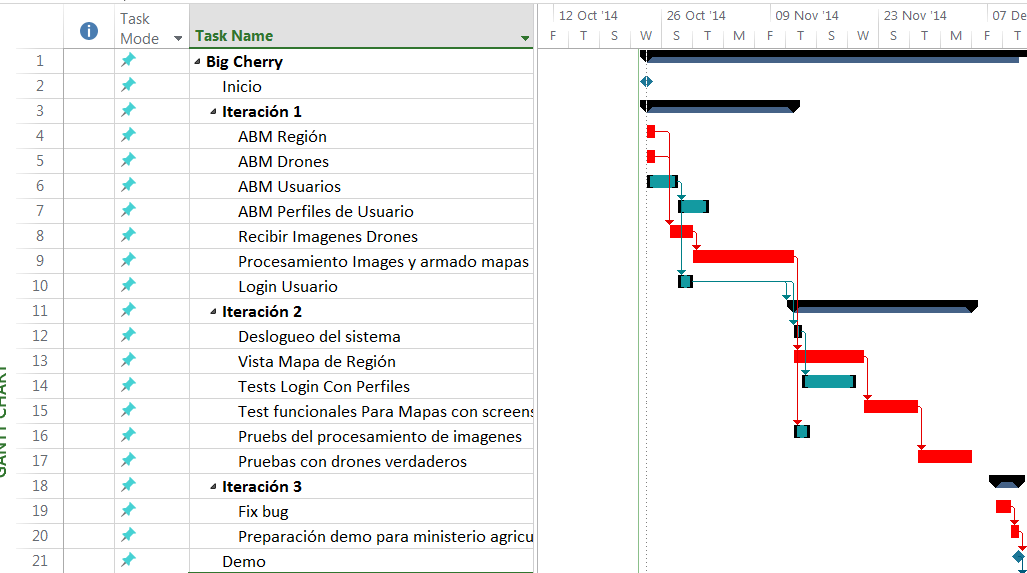
\includegraphics[width=1\textwidth]{demo.png}
  \caption{Diagrama Con las Iteraciones para la demo}
  \label{fig:clases4}
\end{figure}

\begin{figure}[h!]
  \centering
  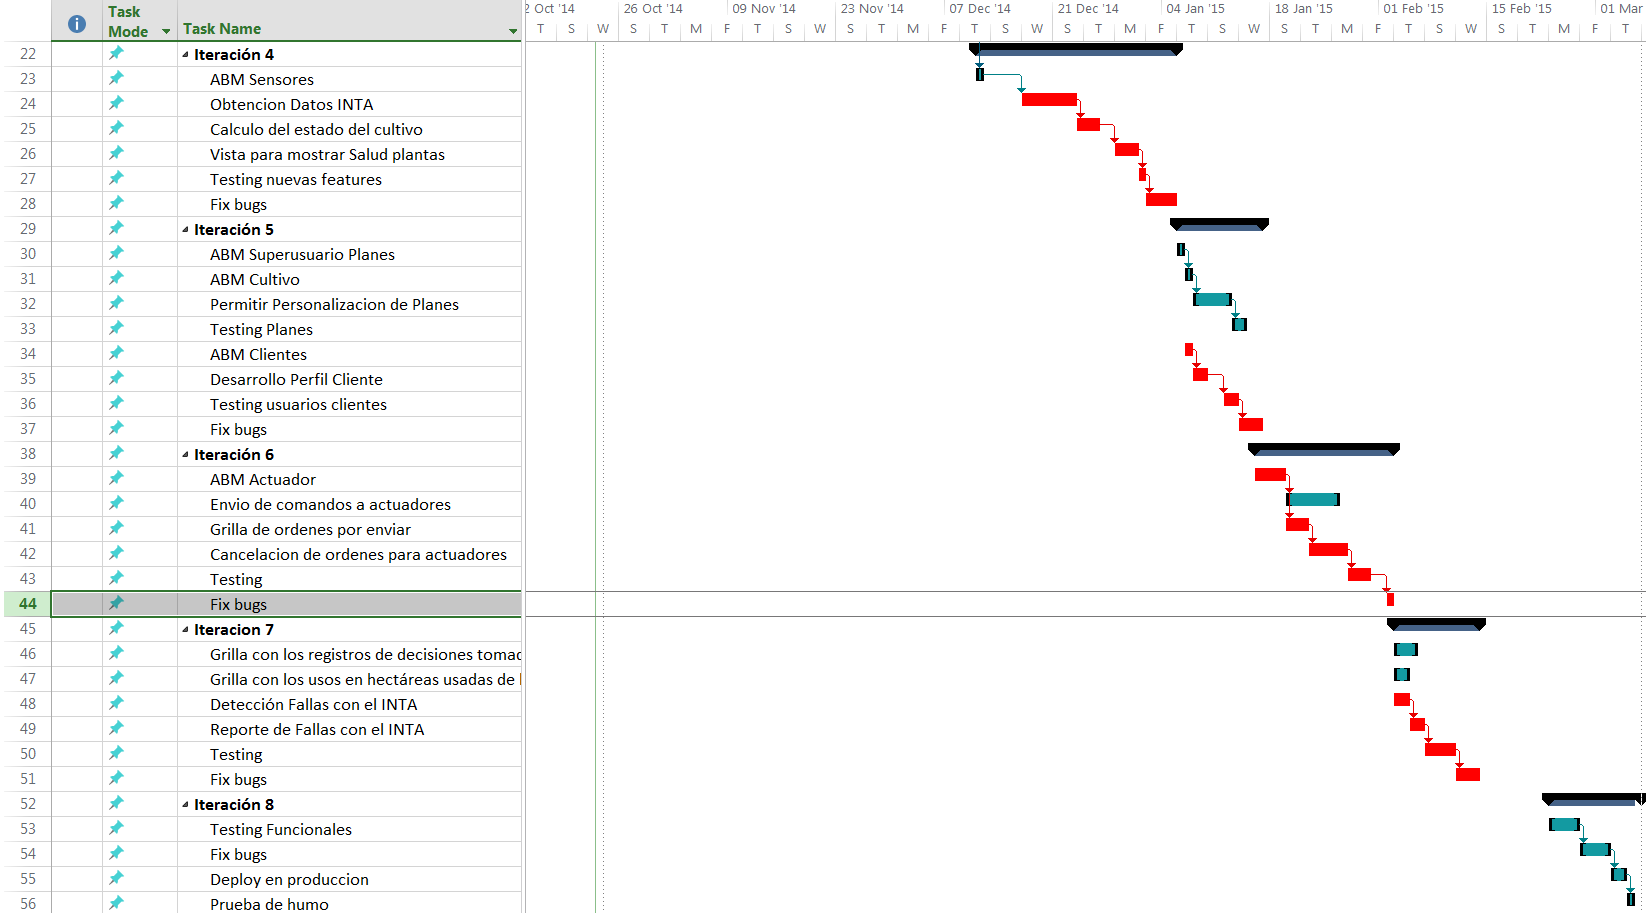
\includegraphics[width=1\textwidth]{ult.png}
  \caption{Diagrama Con las Iteraciones posteriores a la demo}
  \label{fig:clases4}
\end{figure}


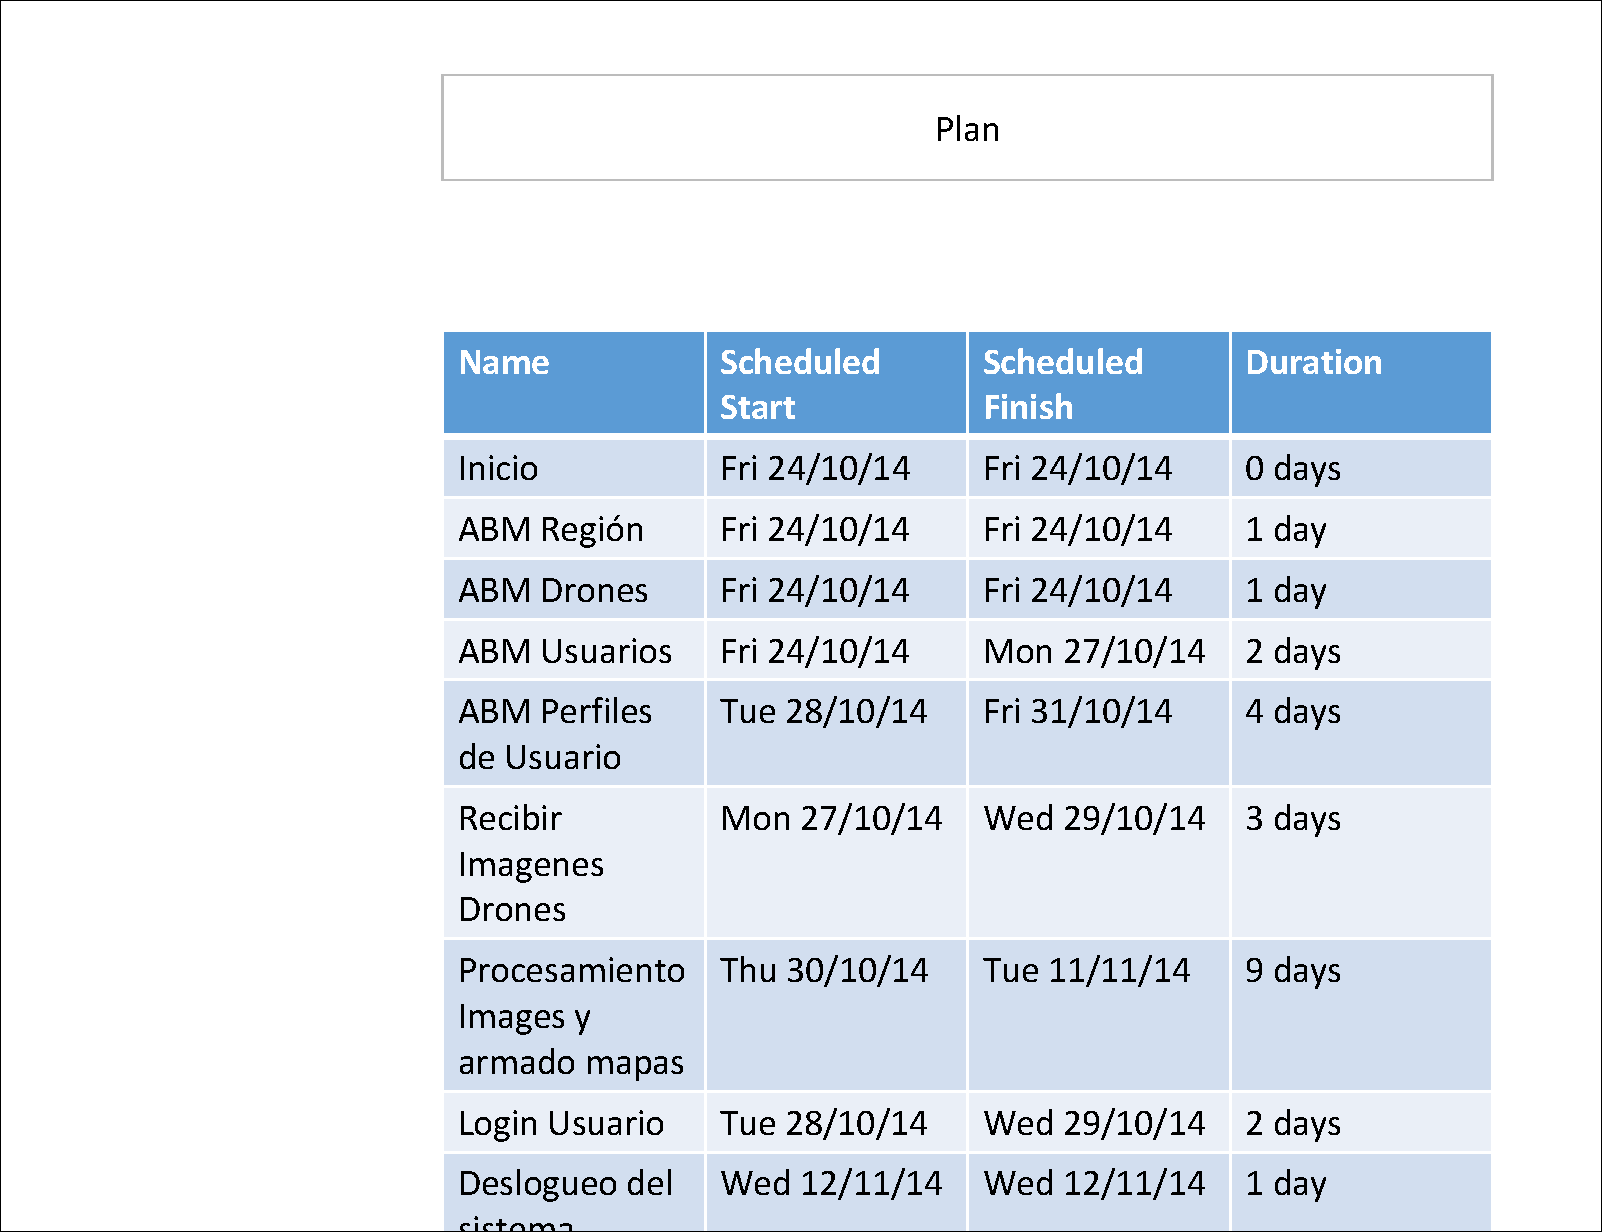
\includepdf[pages={1}]{plan.pdf}
\includepdf[pages={2}]{plan.pdf}
\includepdf[pages={3}]{plan.pdf}
\includepdf[pages={4}]{plan.pdf}
\includepdf[pages={5}]{plan.pdf}
\section{Introducción}

En el presente trabajo se aborda la extensión del diseño presentado en el TP1, debiendo ahora plantear un sistema de cultivo de muchas plantas en grandes extensiones de terreno y para muchos clientes. Dada esta nueva situación, aparecen varios stakeholders que, por su colaboración en el proyecto proveyendo logística o servicios, o por su intención de consumo, imponen distintos requerimientos que sumados a los técnicos desembocan en la contemplación de diversos riesgos y atributos de calidad.\\
Aquí se presenta una planificación de las fases de \textit{elaboración} y \textit{construcción} de la metodología UP, asumiendo que la fase \textit{inception} ya se ha desarrollado. En esta primera etapa se han presentado las ideas para la formulación del proyecto BigCherry, se han establecido los requerimientos y recursos disponibles, y se ha llevado a cabo el QAW del cual se desprendieron algunos atributos de calidad esperados en el producto final.

\section{Casos de Uso}

\subsection{Asignación de CU}

Para comenzar a trabajar sobre la planificación del proyecto se identificó un conjunto de casos de uso que cubriera la mayoría de las funcionalidades que se desprenden de los requerimientos obtenidos. Los mismos se organizaron en seis iteraciones, distribuidas a lo largo de las fases de elaboración y construcción de la metodología UP. La división de los CU en las distintas iteraciones y la organización de las mismas estuvo pautada por las necesidades manifestadas por los stakeholders y un incremento de funcionalidad, partiendo del núcleo más importante y revistiendo la aplicación a lo largo del tiempo de lógica menos prioritaria.\\
\indent Dado que la primera iteración ya contaba con un tiempo fijado (3 semanas), se determinó trabajar en este tiempo en la comunicación con la red pública de drones (ya que el Ministerio exigía que esto estuviera implementado en los primeros dos meses), la recepción y procesamiento de las imágenes, la traducción de estos datos en mediciones de los indicadores de estado de los cultivos y una mínima interacción con actuadores. Para las siguientes iteraciones se adjudicaron casos de uso que totalizaran una cantidad de tiempo similar y que implicaran una evolución coherente y funcional de la aplicación. Por ejemplo, para la segunda iteración se asignaron los casos de uso relacionados con la programación de seguimiento de cultivos, el monitoreo de la salud de las plantas y la comunicación con las estaciones climatológicas, mientras que la encrptación de datos se diagramó en la órbita de la sexta y última iteración.\\
\indent Parte de este cronograma fue también regido por el análisis de riesgos, presentado en la \textbf{SECCION}, el cual se vio alimentado por los requerimientos iniciales y por las intervenciones de los distintos stakeholders en el QAW. De esta manera, dado que el riesgo más importante resultó ser la correcta implementación de la comunicación con la red pública de drones, se decidió incluir este desarrollo dentro de la primera iteración, de casi un mes de duración, para garantizar que haya el suficiente tiempo para llevar adelante esta tarea dentro del marco de tiempo requerido.

\clearpage

\subsection{Iteraciones}

\textbf{Primera iteración} [3 semanas]
	\begin{enumerate}
		\item Accediendo a la red pública de drones
		\item Recibiendo imágenes de los drones
		\item Procesando datos de bandas espectrales de las fotografías
		\item Interactuando con actuadores
	\end{enumerate}

\textbf{Segunda iteración} [2 semanas]
	\begin{enumerate}
		\item Generando mediciones de estado del terreno / cultivos a partir de fotos procesadas
		\item Monitoreando el estado de salud de las plantas
		\item Obteniendo información del clima a partir de las micro-estaciones climatológicas del INTA.
		\item Calculando decisión según información recolectada y plan maestro
	\end{enumerate}

\textbf{Tercera iteración} [2 semanas]
	\begin{enumerate}
		\item Iniciando seguimiento de cultivos / región
		\item Incorporando nuevas especies de cultivo (ABM Cultivo)
		\item Consultando planes maestros de cultivo provistos por el INTA / organismos privados (ABM Plan)
		\item Consultando estado de los cultivos
		\item Accediendo a la red privada de drones
	\end{enumerate}

\textbf{Cuarta iteración} [2 semanas]
	\begin{enumerate}
		\item Supervisando acciones ordenadas a actuadores
		\item Agregando muestreo manual del estado de los cultivos / terreno
		\item Visualizando el mapa del estado del terreno
		\item Personalizando plan maestro de cultivo
		\item Agregando nuevos actuadores (ABM Actuador)
	\end{enumerate}

\textbf{Quinta iteración} [2 semanas]
	\begin{enumerate}
		\item Logueando eventos del sistema
		\item Autenticando usuario (ABM Usuario)
		\item Autorizando usuario (ABMs Rol y Permiso)
		\item Revisando registro de eventos
	\end{enumerate}

\textbf{Sexta iteración} [2 semanas]
	\begin{enumerate}
		\item Manejando fallas de servidores de INTA
		\item Descargando fotos offline de dron
		\item Organizando información almacenada entre nodos ArSat
		\item Encriptando / desencriptando información a almacenar
	\end{enumerate}

\clearpage

\subsection{Síntesis CU Primera iteración}
		
\begin{enumerate}
	\item \textbf{Accediendo a la red pública de drones}
	Se refiere a la conexión y comunicación con la red estatal de drones. BigCherry debe poder iniciar una sesión dentro de la red y realizar peticiones de imágenes para ciertas coordenadas. Debe poder enviar los mensajes acorde a la especificación de la API de la red y a su vez debe poder interpretar los distintos mensajes que ésta le envía, sean de comportamiento normal o error. Esto debe permitir, además, la parametrización de los pedidos y el acceso a otros datos de los drones como disponibilidad, tiempo estimado de envío de la información, etc.

	\item \textbf{Recibiendo imágenes de los drones}
	Una vez satisfecho el pedido de imágenes aéreas, el sistema debe poder recibir las mismas sin errores y almacenarlas correctamente para su posterior procesamiento. Es importante que pueda manejar la recepción de muchas imágenes en simultáneo y que esto no afecte transimisión de otros datos con el resto de los drones.

	\item \textbf{Procesando datos de bandas espectrales de las fotografías}
	Al analizar las imágenes se deben aplicar distintos filtros para obtener datos del suelo como temperatura, humedad, salinidad del agua y otros indicadores pertinentes a la salud de las plantas. Ademśas se deben determinar posibles problemas como fotografías corruptas, mal tomadas (con obstáculos) o que presenten otro tipo de anomalías. La salida de este procesamiento debe almacenarse acorde al input procesado para posteriores consultas.

	\item \textbf{Interactuando con actuadores} 
	Este CU refiere a la interacción de BigCherry con los actuadores registrados, ya sean pulverizadoras, cosechadoras, sistemas de riego o fertilización, etc. Deben poder enviarse mensajes con directivas para que éstos lleven a cabo a través del protocolo de comunicación que maneje cada dispositivo.
\end{enumerate}

\subsection{Detalle Primera iteración}

\begin{itemize}
\item Identificación: E1
\item Tipo de iteración: Elaboración
\item Tareas:
	\begin{enumerate}
	\item Refinamiento de objetivos y requerimientos
	\item QAW con stakeholders y equipo
	\item Análisis de riesgos
	\item Reconocimiento de casos de uso
	\item División de CU en iteraciones según prioridad
	\item Estimación de tiempos de CU
	\item Análisis de escenarios y atributos de calidad del sistema
	\item Diseño de arquitectura
	\item Realización de tareas de CU1
	\item Realización de tareas de CU2
	\item Realización de tareas de CU3
	\item Realización de tareas de CU4	
	\end{enumerate}
\end{itemize}


\section{Análisis de Riesgos}

\textbf{Interfaz con los drones en dos meses}
\begin{itemize}
 \item \textsl{Descripci\'on}: 
 \item \textsl{Probabilidad}: 
 \item \textsl{Impacto}: 
 \item \textsl{Exposición}: 
 \item \textsl{Mitigación}: 
 \item \textsl{Plan de Contingencia} : 
\end{itemize}
\textbf{Disponibilidad usando la red estatal}
\begin{itemize}
 \item \textsl{Descripci\'on}: 
 \item \textsl{Probabilidad}: 
 \item \textsl{Impacto}: 
 \item \textsl{Exposición}: 
 \item \textsl{Mitigación}: 
 \item \textsl{Plan de Contingencia} : 
\end{itemize}
\textbf{Servidores del INTA inestables}
\begin{itemize}
 \item \textsl{Descripci\'on}: 
 \item \textsl{Probabilidad}: 
 \item \textsl{Impacto}: 
 \item \textsl{Exposición}: 
 \item \textsl{Mitigación}: 
 \item \textsl{Plan de Contingencia} : 
\end{itemize}
\textbf{Demasiado volumen de informaci\'on }
\begin{itemize}
 \item \textsl{Descripci\'on}: 
 \item \textsl{Probabilidad}: 
 \item \textsl{Impacto}: 
 \item \textsl{Exposición}: 
 \item \textsl{Mitigación}: 
 \item \textsl{Plan de Contingencia} : 
\end{itemize}
\textbf{Uso de servidores p\'ublicos}
\begin{itemize}
 \item \textsl{Descripci\'on}: 
 \item \textsl{Probabilidad}: 
 \item \textsl{Impacto}: 
 \item \textsl{Exposición}: 
 \item \textsl{Mitigación}: 
 \item \textsl{Plan de Contingencia} : 
\end{itemize}
\textbf{Auditabilidad en todas las decisiones tomadas para validar imparcialidad}
\begin{itemize}
 \item \textsl{Descripci\'on}: 
 \item \textsl{Probabilidad}: 
 \item \textsl{Impacto}: 
 \item \textsl{Exposición}: 
 \item \textsl{Mitigación}: 
 \item \textsl{Plan de Contingencia} : 
\end{itemize}
\textbf{zonas relefadas por motivos politicos alegando motivos t\'ecnicos}
\begin{itemize}
 \item \textsl{Descripci\'on}: 
 \item \textsl{Probabilidad}: 
 \item \textsl{Impacto}: 
 \item \textsl{Exposición}: 
 \item \textsl{Mitigación}: 
 \item \textsl{Plan de Contingencia} : 
\end{itemize}

\textbf{Errores en las comunicaciones}
\begin{itemize}
 \item \textsl{Descripci\'on}: Pueden surgir errores en la comunicación con los servidores del \textbf{INTA}
 \item \textsl{Probabilidad}: Media
 \item \textsl{Impacto}: Media
 \item \textsl{Exposición}: Media
 \item \textsl{Mitigación}: Detectar fallas en la comunicación para poder reportar y seguir con el normal funcionamineto.
 \item \textsl{Plan de Contingencia} : Utilizar informaci\'on de sensores e imágenes de drones para poder calcular resultados similares a los del \textbf{INTA}.
\end{itemize}

\textbf{Cobertura de conexión}
\begin{itemize}
 \item \textsl{Descripci\'on}: Problemas de conectividad en zonas sin acceso a internet u otras redes de comunicación.
 \item \textsl{Probabilidad}: Alta
 \item \textsl{Impacto}: Media
 \item \textsl{Exposición}: Media
 \item \textsl{Mitigación}: El sistema llevaría un historial con fecha de datos externos y detectaría cuándo los datos son viejos usando un reloj interno.
 \item \textsl{Plan de Contingencia}: Permitir la carga manual de datos por medio de importación de archivos u otras fuentes.
\end{itemize}

\textbf{Vulnerabilidades en la seguridad}
\begin{itemize}
 \item \textsl{Descripci\'on}: Cliente puede ver datos de otro cliente.
 \item \textsl{Probabilidad}: Baja
 \item \textsl{Impacto}: Alto
 \item \textsl{Exposición}: Media
 \item \textsl{Mitigación}: Realizar test para probar casos de borde con los cuentas de clientes. Pagar a una consultora de seguridad para pruebas tercerizadas.
 \item \textsl{Plan de Contingencia}: Permitir el apagado rápido del sistema en caso de detecci\'on de problemas de seguridad. Guardar en logs las operaciones realizadas para cada dominio / cliente / empresa.
\end{itemize}

\textbf{Aumento de costos por utilizar la red privada de drones}
\begin{itemize}
 \item \textsl{Descripci\'on}: Se utiliza mucho la red privada de drones en vez de la pública.
 \item \textsl{Probabilidad}: Media
 \item \textsl{Impacto}: Alto
 \item \textsl{Exposición}: Alto
 \item \textsl{Mitigación}: El sistema calcularía cada cierto intervalo el consumo por hect\'areas.
 \item \textsl{Plan de Contingencia} : Desactivar la red privada en caso de susperar algún límite de uso diario, mensual, etc. Enviar alertar al administrador del sistema. Si no logra acceder a la red pública pasa al caso de falta de conectividad y se aplica el plan 
\end{itemize}

\clearpage

\textbf{Delays en accionar de actuadores}
\begin{itemize}
 \item \textsl{Descripci\'on}: Demora al enviar acciones a los actuadores.
 \item \textsl{Probabilidad}: Media
 \item \textsl{Impacto}: Alta
 \item \textsl{Exposición}: Alta
 \item \textsl{Mitigación}: En el sistema se usarán actuadores que confirman la recepci\'on de acciones.
 \item \textsl{Plan de Contingencia}: Se chequeará que las acciones fueron recibidas por los actuadores y en caso de timeout se reenviarán. Ante la primera falla se le avisar\'a al administrador / encargado.
\end{itemize}

\textbf{Problemas con almacenamiento}
\begin{itemize}
 \item \textsl{Descripci\'on}: Volumen de informaci\'on muy grande.
 \item \textsl{Probabilidad}: Media
 \item \textsl{Impacto}: Alto
 \item \textsl{Exposición}: Alto
 \item \textsl{Mitigación}: Utilizar algoritmos para comprimir los datos.
 \item \textsl{Plan de Contingencia}: Monitorear el trafico de la red y espacio de disco en los nodos de \textbf{ArSAT}. Rediseñar parte de la persistencia para evitar redundancia de datos innecesaria.
\end{itemize}


\end{document}
